\documentclass[12pt]{article}
\usepackage{setspace}
\doublespacing
\usepackage{times}
\usepackage{natbib}
\usepackage{fullpage}
\usepackage{tikz}
\usepackage{amsmath,amssymb}
\usepackage{hyperref}
\usepackage{graphicx}
\usepackage{algorithmic}
\usepackage{multirow}

\DeclareMathOperator*{\argmin}{arg\,min}
\DeclareMathOperator*{\Lik}{Lik}
\DeclareMathOperator*{\PoissonLoss}{PoissonLoss}
\DeclareMathOperator*{\Peaks}{Peaks}
\DeclareMathOperator*{\Segments}{Segments}
\DeclareMathOperator*{\argmax}{arg\,max}
\DeclareMathOperator*{\maximize}{maximize}
\DeclareMathOperator*{\minimize}{minimize}
\newcommand{\sign}{\operatorname{sign}}
\newcommand{\keyword}[1]{\textbf{#1}}
\newcommand{\RR}{\mathbb R}
\newcommand{\ZZ}{\mathbb Z}
\newcommand{\NN}{\mathbb N}

\begin{document}

\title{Introduction to machine learning and neural networks}

\author{
  Toby Dylan Hocking\\
  toby.hocking@nau.edu
}

\maketitle


% Your manuscript is 20 or fewer pages, double space, including figures and tables, for each lecture or practice. That makes about 10 book pages. Exception is possible for a few lectures.

% Each manuscript may include 3-5 illustrations.

% Manuscript should be written at a level to be understood by first-year graduate students. 

% Each manuscript has a short, first paragraph (<50 words) about the training goal.

% Do not have too many references as it is not a research paper but list a few suggested readings.

% Include a few (4-6) quizzes for each lecture and expected homework for each practice.

% Text in your chapter should be corresponding to the pre-recorded video or the video to be recorded.

\paragraph{Objective.} In this chapter we introduce basic concepts and
algorithms from machine learning. We explain how neural networks can
be used for regression and classification problems, and how
cross-validation can be used for training and testing machine learning
algorithms.

\section{Introduction and applications of machine learning}

Machine learning is the domain of computer science which is concerned
with efficient algorithms for making predictions in all kinds of big
data sets. A defining characteristic of supervised machine learning
algorithms is that they require a data set for training. The machine
learning algorithm then memorizes the patterns present in those
training data, with the goal of accurately predicting similar patterns
in new test data. Many machine learning algorithms are
domain-agnostic, which means they have been shown to provide highly
accurate predictions in a wide variety of application domains
(computer vision, speech recognition, automatic translation, biology,
medicine, climate science, chemistry, geology, etc). 

\begin{figure} 
  \centering
  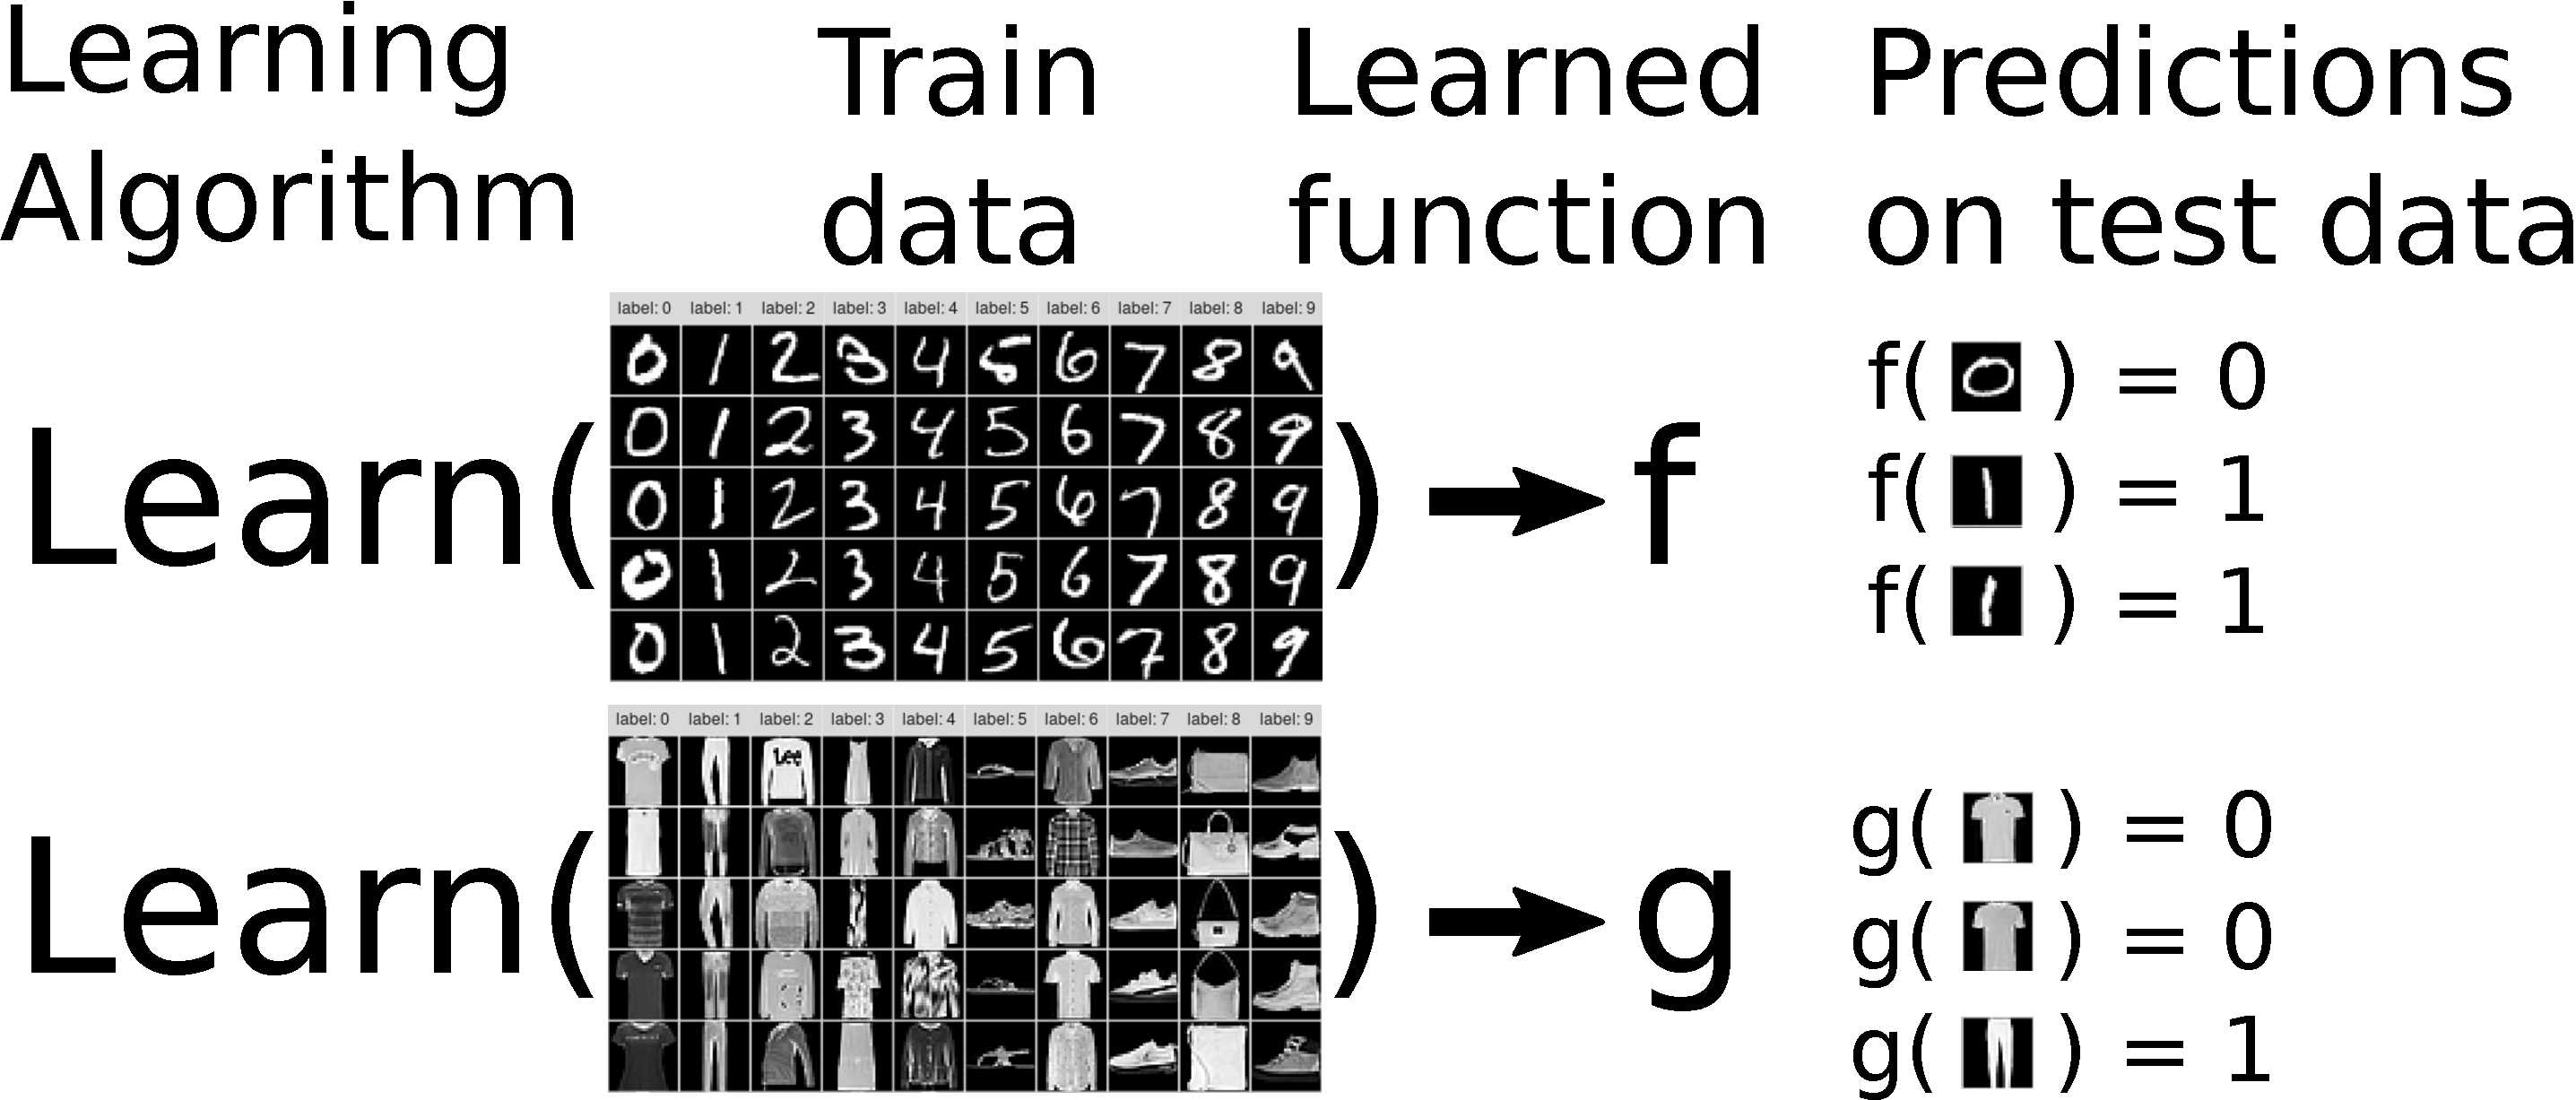
\includegraphics[width=0.8\textwidth]{drawing-mnist-train-test.pdf}
  \caption{A learning algorithm inputs a train data set, and outputs a
    prediction function, g or h. Both g and h input a grayscale image
    and output a class (integer from 0 to 9), but g is for  
    digits and h is for fashion.}
  \label{fig:drawing-mnist-train-test}
\end{figure}

For example, consider the problem of image classification from the
application domain of computer vision. In this problem, we would like
a function that can input an image, and output an integer which
indicates class membership. More precisely, let us consider the MNIST
and Fashion-MNIST data sets
(Figure~\ref{fig:drawing-mnist-train-test}), in which each input is
grayscale image with height and width of 28 pixels, 
represented as a matrix of real numbers
$\mathbf x\in\mathbb R^{28\times 28}$ \citep{LeCun1998,Xiao2017}. In
both the MNIST and Fashion-MNIST data sets each image has a
corresponding label which is an integer $y\in\{0,1,\dots,9\}$. In the
MNIST data set each image/label represents a digit, whereas in
Fashion-MNIST each image/label represents a category of clothing (0
for T-shirt/top, 1 for Trouser, 2 for Pullover, etc).  In both data
sets the goal is to learn a function
$f:\mathbb R^{28\times 28}\rightarrow \{0,1,\dots, 9\}$ which inputs
an image $\mathbf x$ and outputs a predicted class $f(\mathbf x)$
which should ideally be the same as the corresponding label $y$.

As mentioned above, a big advantage of supervised learning algorithms
is that they are typically domain-agnostic, meaning that they can
learn accurate prediction functions $f$ using data sets with different
kinds of patterns. That means we can use a single learning algorithm
\textsc{Learn} on both the MNIST or Fashion-MNIST data sets
(Figure~\ref{fig:drawing-mnist-train-test}, left). For the MNIST data
set the learning algorithm will output a function for predicting the
class of digit images, and for Fashion-MNIST the learning algorithm
will output a function for predicting the class of a clothing image
(Figure~\ref{fig:drawing-mnist-train-test}, right). The advantage of
this supervised machine learning approach to image classification is
that the programmer does not need any domain-specific knowledge about
the expected pattern (e.g., shape of each digit, appearance of each
clothing type). Instead, we assume there is a data set with enough
labels for the learning algorithm to accurately infer the
domain-specific pattern and prediction function. This means that the
machine learning approach is only appropriate when it is
possible/inexpensive to create a large labeled data set that
accurately represents the pattern/function to be learned.

How do we know if the learning algorithm is working properly? The goal
of supervised learning is \keyword{generalization}, which means the
learned prediction function $f$ should accurately predict
$f(\mathbf x) = y$ for any inputs/outputs $(\mathbf x,y)$ that will be
seen in a desired application (including new data that were not seen
during learning). To formalize this idea, and to compute quantitative
evaluation metrics (accuracy/error rates), we need a test data set, as
explained in the next section.

\subsection{$K$-fold cross-validation for evaluating prediction/test accuracy}

Each input $\mathbf x$ in a data set is typically represented as one
of $N$ rows in a design matrix with $D$ columns (one for each
dimension or feature). Each output $y$ is represented as an element of
a label vector of size $N$, which can be visualized as another column
alongside the design matrix (Figure~\ref{fig:cross-validation},
left). For example, in the image data sets discussed above we have
$N=60,000$ labeled images/rows, each with $D=784$ dimensions/features
(one for each of the $28\times 28$ pixels in the image).

The goal of supervised learning is to find a prediction function $f$
such that $f(\mathbf x) = y$ for all inputs/outputs $(\mathbf x,y)$ in
a test data set (which is not available for learning
$f$). So how do we learn $f$ for accurate prediction on a test data
set, if that test set is not available? We must assume that we have
access to a train data set with the same statistical distribution as
the test data. The train data set is used to learn $f$, and the test
data can only be used for evaluating the prediction accuracy/error of
$f$.

Some benchmark data sets which are used for machine learning research,
like MNIST and Fashion-MNIST, have designated train/test
sets. However, in most applications of machine learning to real data
sets, train/test sets must be created. One approach is to create a
single train/test split by randomly assigning a set to each of the $N$
rows/observations, say 50\% train rows and 50\% test rows. The
advantage of that approach is simplicity, but the drawback is that we
can only report accuracy/error metrics with respect to one test set
(e.g., the algorithm learned a function which accurately predicted
91.3\% of observations/labels in the test set, meaning 8.7\% error
rate). 

In addition to estimating the accuracy/error rate, is important to
have some estimate of variance in order to make statements about
whether the prediction accuracy/error of the learned function $f$ is
significantly larger/smaller than other prediction functions. The
other functions to compare against may be from other supervised
learning algorithms, or some other method that does not use machine
learning (e.g., a domain-specific physical/mechanistic model). A common
baseline is the constant function $f(\mathbf x) = y_0$ where $y_0$ is
the average or most frequent label in the train data. This baseline
ignores all of the inputs/features $\mathbf x$, and can be used to
show that the algorithm is learning some non-trivial predictive relationship
between inputs and outputs (for an example see
Figure~\ref{fig:test-accuracy}).

\begin{figure}
  \centering
  \includegraphics[width=\textwidth]{drawing-cross-validation}
  \caption{$K=3$ fold cross-validation. \textbf{Left:} the first step
    is to randomly assign a fold ID from 1 to $K$ to each of the
    observations/rows. \textbf{Right:} in each of the
    $k\in\{1, \dots, K\}$ splits, the observations with fold ID $k$
    are set aside as a test set, and the other observations are used
    as a train set to learn a prediction function (f1--f3), which is
    used to predict for the test set, and to compute accuracy metrics
    (A1--A3).}
  \label{fig:cross-validation}
\end{figure}

The $K$-fold cross-validation procudure generates $K$ splits, and can
therefore be used to estimate both mean and variance of prediction
accuracy/error. The number of folds/splits $K$ is a user-defined
integer parameter which must be at least 2, and at most $N$. Typical
choices range from $K=3$ to 10, and usually the value of $K$ does not
have a large effect on the final estimated mean/variance of prediction
accuracy/error. The algorithm begins by randomly assigning a fold ID
number (integer from 1 to $K$) to each observation
(Figure~\ref{fig:cross-validation}, left). Then for each unique fold
value from 1 to $K$, we hold out the corresponding observations/rows
as a test set, and use data from all other folds as a train set
(Figure~\ref{fig:cross-validation}, right). Each train set is used to
learn a corresponding prediction function, which is then used to
predict on the held out test data. Finally, accuracy/error metrics are
computed in order to quantify how well the predictions fit the labels
for the test data. Overall for each data set and learning algorithm
the $K$-fold cross-validation procedure results in $K$ splits, $K$
learned functions, and $K$ test accuracy/error metrics, which are
typically combined by taking the mean and standard deviation (or
median and quartiles). Other algorithms may be used with the same fold
assignments, in order to compare algorithms in terms of accuracy/error
rates in particular data sets.

For example, Figure~\ref{fig:test-accuracy} uses $K=4$-fold
cross-validation to compare four learned functions on an image
classification problem. The accuracy rates of the ``dense'' and
``linear'' functions, $97.4 \pm 1.6 \%$ and $96.3 \pm 1.9 \%$ (mean
$\pm$ standard deviation) are not significantly different. Both rates
are significantly larger than the accuracy of the ``baseline''
constant function, $16.4 \pm 1.4 \%$, and smaller than the accuracy of
the ``conv'' function, $99.3 \pm 1.1 \%$. We can therefore conclude
that the most accurate learning algorithm for this problem, among
these four candidates, is the ``conv'' method (which uses a
convolutional neural network, explained later).  It is important to
note that statements about what algorithm is most accurate only makes
sense in terms of a particular data set, after having performed
$K$-fold cross-validation to estimate prediction accuracy/error rates.

\subsection{Other applications}

So far we have only discussed machine learning algorithms in the
context of a single prediction problem, image classification. In this
section we briefly discuss other applications of machine learning. In
each application the set of possible inputs $\mathbf x$ and outputs
$y$ are different, but machine learning algorithms can always be used
to learn a prediction function $f(x)\approx y$. 

\citep{Jones2009} proposed to use interactive machine learning for
cell image classification in the CellProfiler Analyst system. This
application is similar to the previously discussed digit/fashion
classification problem, but with only two classes (binary
classification). In this context the input is a multi-color image of
cell $\mathbf x\in\mathbb R^{h \times w \times c}$ where $h,w$ are the
height and width of the image in pixels, and $c=3$ is the number of
channels used to represent a color image (red, green, blue). The
output $y\in\{0,1\}$ is a binary label which indicates whether or not
the image contains the cell phenotype of interest. 

Some email programs use machine learning for spam filtering, which is
another example of a binary classification problem. When you click the
``spam'' button in the email program you are labeling that email as
spam ($y=1$), and when you respond to an email you are labeling that
email as not spam ($y=0$). The input $\mathbf x$ is an email message,
which can be represented using a ``bag-of-words'' vector (each element
is the number of times a specific word occurs in that email message).

\citet{Russell2008} proposed the LabelMe tool for creating data sets
for image segmentation, which is more complex than the previously
discussed image classification problems. In this context the input
$\mathbf x\in\mathbb R^{h \times w \times c}$ is typically a
multi-color image, and the output
$\mathbf y\in \{0,1\}^{h \times w}$ is a binary mask (one element
for every pixel in the image) indicating whether or not that pixel
contains an object of interest.

Machine learning can be used for automatic translation between
languages. In this context the input is a text in one language (e.g.,
French) and the output is the text translated to another language
(e.g., English). The desired prediction function $f$ inputs a French
text and outputs the English translation.

Machine learning can be used for medical diagnosis. For example
\citet{Poplin2017} showed that retinal photographs can be used to
predict blood pressure or risk of heart attack. Since the output $y$
is a real number (e.g., blood pressure of 120 mm mercury), we refer to
this as a regression problem.

\section{Avoiding under/overfitting in a neural network for regression}

Now we consider a simple regression problem for which the input
$x\in\mathbb R$ is a single real number ($D=1$ feature/column in the
design matrix), and the output $y\in\mathbb R$ is as well. Using a
neural network with a single hidden layer of $U$ units, there are two
unknown \keyword{parameter} vectors which need to be learned using the training
data, $\mathbf w\in \mathbb R^U$ and $\mathbf v\in \mathbb R^U$. The prediction
function $f$ is then defined as
\begin{equation}
  f(x) = \mathbf w^\intercal \sigma( x \mathbf v ) = \mathbf w^\intercal \mathbf z,
\end{equation}
where $\sigma:\mathbb R^U\rightarrow \mathbb R^U$ is a non-linear
activation function, and $\mathbf z\in \mathbb R^U$ is the vector of
hidden units. Typical activation functions include the logistic
sigmoid $\sigma(t)=1/(1+\exp(-t))$ and the rectifier (or rectified
linear units, ReLU) $\sigma(t)=\max(0, t)$. The prediction function is
learned using gradient descent, which is an algorithm that attempts to
find parameters $\mathbf w,\mathbf v$ which minimize the mean squared
error between the predictions and the corresponding labels in the $N$
train data,
\begin{equation}
  \mathcal L(\mathbf w, \mathbf v) = \frac{1}{N} \sum_{i=1}^N [ \mathbf w^\intercal \sigma( x_i \mathbf v ) - y_i ]^2. \label{eq:loss}
\end{equation}
Gradient descent begins using un-informative parameters
$\mathbf w_0,\mathbf v_0$ (typically random numbers close to zero),
then at each iteration $t\in\{1,\dots, T\}$ the parameters are
improved by taking a step of size $\alpha>0$ in the negative gradient
direction,
\begin{eqnarray}
  \mathbf w_t &=& \mathbf w_{t-1} - \alpha \nabla_{\mathbf w} \mathcal L(\mathbf w, \mathbf v),\\
  \mathbf v_t &=& \mathbf v_{t-1} - \alpha \nabla_{\mathbf v} \mathcal L(\mathbf w, \mathbf v).
\end{eqnarray}
The algorithm described above is referred to as ``full gradient''
because the gradient is defined using the full set of $N$ samples in
the train set. Other common variants include ``stochastic gradient''
(gradient uses one sample) and ``minibatch'' (gradient uses several
samples). When doing gradient descent on a neural network model, one
``epoch'' includes computing gradients once for each sample (e.g., 1
epoch = 1 iteration of full gradient, 1 epoch = $N$ iterations of
stochastic gradient).

In the algorithm above, the number of hidden units $U$, the number of
iterations $T$, and the step size $\alpha$ must be fixed before
running the learning algorithm. These \keyword{hyper-parameters}
affect the learning capacity of the neural network.  An important
consideration when using any machine learning algorithm is that you
most likely need to tune the hyper-parameters of the algorithm in
order to avoid underfitting and overfitting. \keyword{Underfitting}
occurs when the learned function $f$ neither provides accurate
predictions for the train data, nor the test
data. \keyword{Overfitting} occurs when the learned function $f$ only
provides accurate predictions for the train data (and not for the test
data). Both underfitting and overfitting are bad, and need to be
avoided, because the goal of any learning algorithm is to find a
prediction function $f$ which provides accurate predictions in test
data.

\begin{figure}
  \centering
  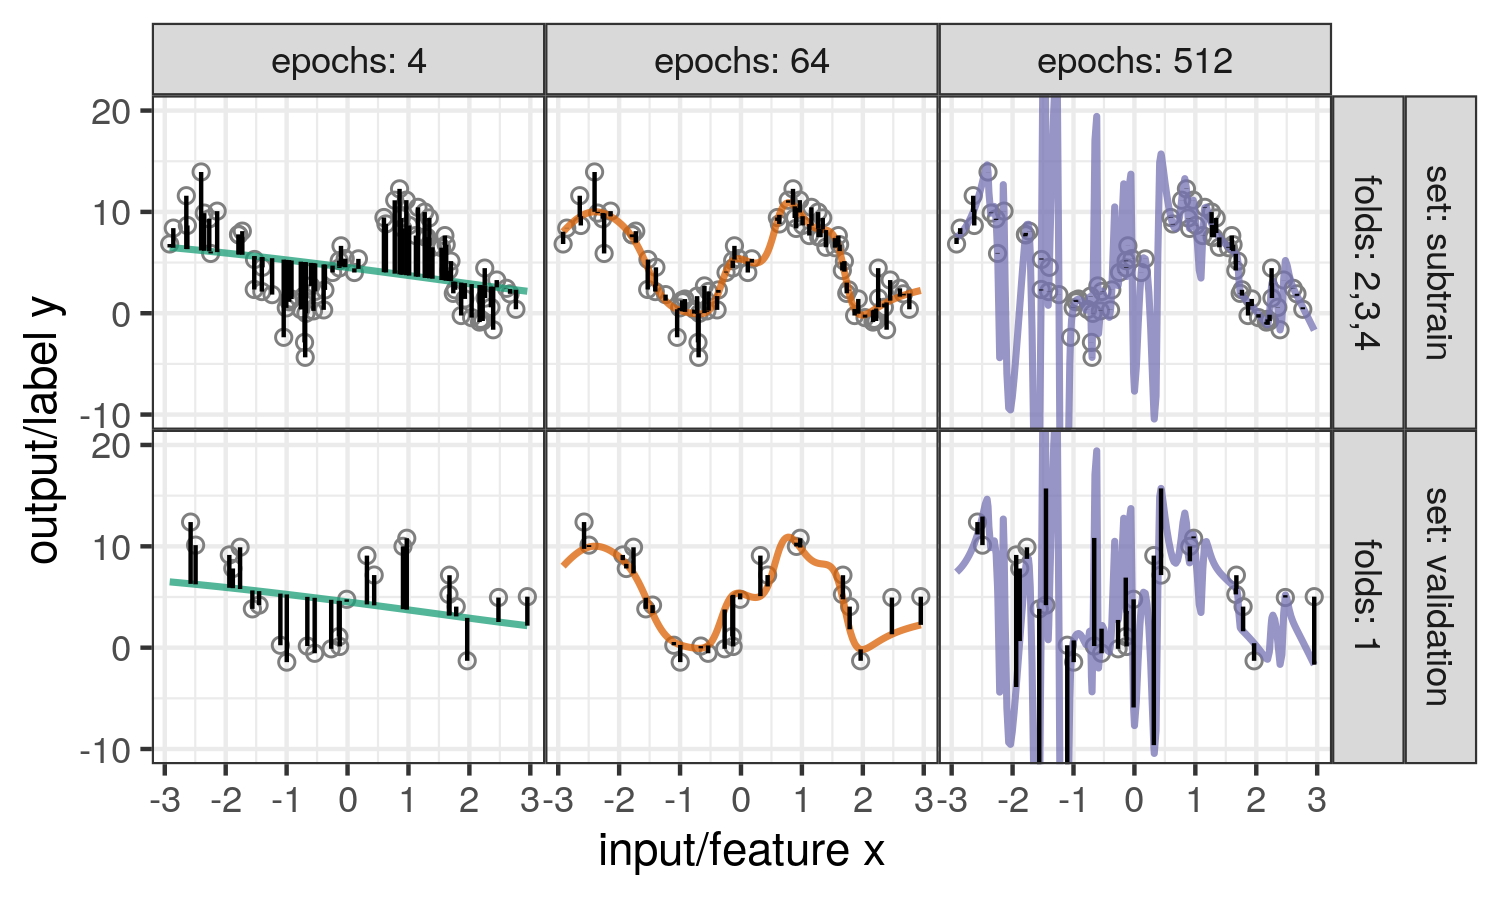
\includegraphics[width=0.55\textwidth]{figure-overfitting-paper}
  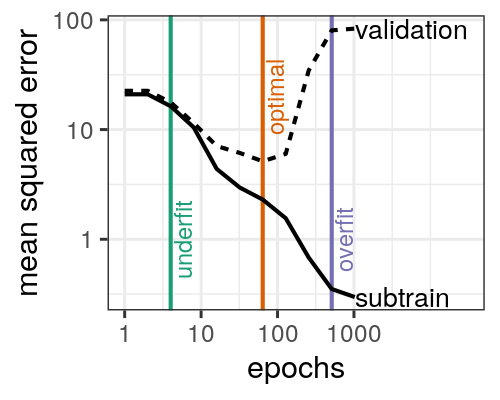
\includegraphics[width=0.4\textwidth]{figure-overfitting-paper-loss}   
  \caption{Illustration of underfitting and overfitting in a neural
    network regression model (single hidden layer, 50 hidden
    units). \textbf{Left:} noisy data with a nonlinear sine wave
    pattern (grey circles), learned functions (colored curves), and
    residuals/errors (black line segments) are shown for three values
    of epochs (panels from left to right) and two data subsets (panels
    from top to bottom). \textbf{Right:} in each epoch the model
    parameters are updated using gradient descent with respect to the
    subtrain loss, which decreases with more epochs. The
    optimal/minimum loss with respect to the validation set occurs at
    64 epochs, indicating underfitting for smaller epochs (green
    function, too regular/linear for both subtrain/validation sets)
    and overfitting for larger epochs (purple function, very
    irregular/nonlinear so good fit for subtrain but not validation
    set).}
  \label{fig:overfitting-paper}
\end{figure}

How can we select hyper-parameters which avoid overfitting? Note that
the choice of hyper-parameters such as number of hidden units $U$ and
iterations $T$ affect the learned function $f$, so we can not use the
test data to learn these hyper-parameters (by assumption that the test
data are not available at train time). Then how do we know which
hyper-parameters will result in learned functions which best
generalize to new data?

A general method which can be used with any learning algorithm is
splitting the train set into subtrain and validation sets, then using
grid search over hyper-parameter values. The subtrain set is used for
parameter learning, and the validation set is used for hyper-parameter
selection. In detail, we first fix a set of hyper-parameters, say
$U=50$ hidden units and $T=100$ iterations. Then the subtrain set is
used with these hyper-parameters as input to the learning algorithm,
which outputs the learned parameter vectors $\mathbf w, \mathbf
v$. Finally the learned parameters are used to compute predictions
$f(x)$ for all inputs $x$ in the validation set, and the corresponding
labels $y$ are used to evaluate the accuracy/error of those
predictions. The procedure is then repeated for another
hyper-parameter set, say $U=10$ hidden units with $T=500$
iterations. In the end we select the hyper-parameter set with minimal
validation error, and then retrain using the learning algorithm on the
full train set with those hyper-parameters. A variant of this method
is to use $K$-fold cross-validation to generate $K$
subtrain/validation splits, then compute mean validation error over
the $K$ splits, which typically yields hyper-parameters that result in
more accurate/generalizable predictions (when compared to
hyper-parameters selected using a single subtrain/validation
split). Note that this $K$-fold cross-validation for hyper-parameter
learning is essentially the same procedure as shown in
Figure~\ref{fig:cross-validation}, but we split the train set
into subtrain/validation sets (instead of splitting all data into
train/test sets as shown in the figure).

For example we simulated some data with a sine wave pattern
(Figure~\ref{fig:overfitting-paper}), and used the R package
\texttt{nnet} to fit a neural network with one hidden layer of $U=50$
units \citep{Ripley2002}. We demonstrate the effects of
under/overfitting by varying the number of iterations/epochs from
$T=1$ to 1000. In this example $K=4$-fold cross-validation was used,
so each data point was randomly assigned a fold ID integer from 1 to
4. The result for only the first split is shown, so observations
assigned fold ID=1 are considered the validation set, and other
observations (folds 2--4) are considered the subtrain set. The data
exhibit a non-linear sine wave pattern, but the learned function for
$T=4$ iterations/epochs is mostly linear (underfitting, large error on
both subtrain/validation sets). For $T=512$ iterations/epochs the
learned function is highly non-linear (overfitting, small error for
the subtrain set but large error for the validation set). When the
error rates are plotted as a function of a model complexity
hyper-parameter such as $T$ (Figure~\ref{fig:overfitting-paper},
right), we see the characteristic U shape for the validation error,
and the monotonic decreasing train error. The hyper-parameter with
minimal validation error is $T=64$ iterations/epochs; smaller $T$
values underfit or are overly regularized, and larger $T$ values
overfit or are under-regularized.

Overall in this section we have seen how a neural network for
regression can be trained using gradient descent (for learning
parameter vectors, given fixed hyper parameters) and
subtrain/validation splits (for learning hyper-parameter values to
avoid under/overfitting).

\section{Comparing neural networks for image classification}

In this section we provide a comparison of
several other neural networks for image classification. In general in
a neural network with $L-1$ hidden layers we can represent the
prediction function as the composition of $L$ intermediate $f_l$
functions, for all layers $l\in\{1,\dots,L\}$:
\begin{equation}
  f(\mathbf x) = f_L[\cdots f_1[\mathbf x] ].
\end{equation}
Each of the intermediate functions has the same form,
\begin{equation}
  f_l(t) = A_l( \mathbf W_l^\intercal t ),
\end{equation}
where $A_l$ is an activation function and
$\mathbf W_l\in\mathbb R^{u_{l}\times u_{l-1}}$ is a weight matrix with
elements that must be learned based on the data. This model includes
several hyper-parameters which must be fixed prior to learning the
neural network weights:
\begin{itemize}
\item The number of layers $L$.
\item The activation functions $A_l$.
\item The number of units per layer $u_l$.
\item The sparsity pattern in the weight matrices $\mathbf W_l$.
\end{itemize}
The number of units in the input layer is fixed, $u_0=D$, based on the
dimension of the inputs $\mathbf x\in\mathbb R^D$. The number of units
in the output layer $u_L$ is also fixed based on the outputs/labels
$y$. The numbers of units in the hidden layers ($u_1,\dots,u_{L-1}$)
are hyper-parameters which control under/overfitting. Increasing the
numbers of hidden units $u_l$ results in larger weight matrices
$\mathbf W_l$, which in general means more parameters to learn, and
larger capacity for fitting complex patterns in the data. The sparsity
pattern of $\mathbf W_l$ means which entries are forced to be zero;
this technique is used in ``convolutional'' neural networks for
avoiding overfitting and reducing training/prediction time. When the
matrix is not sparse (all entries non-zero), we refer to the layer as
dense or fully connected.

For example in the previous section we used a neural network for
regression with one hidden layer, which in this more general notation
means using $L=2$ intermediate functions; the input dimension is
$u_0=D=1$, the number of hidden units is $u_1=U=50$, and there is a
single output $u_2=1$ to predict. The weight matrices are dense/fully connected (no convolution/sparsity), of
dimension
$\mathbf W_1\in\mathbb R^{50\times 1}, \mathbf W_2\in\mathbb R^{1
  \times 50}$. The hidden layer
activation function $A_1$ used by the R \texttt{nnet} package is the
logistic sigmoid, $\sigma(t)=1/(1+\exp(-t))$, and the output
activation for regression (real-valued outputs) is the identity,
$A_2(t)=t$.

In this section we implement three other neural networks for image
classification. Using the ``zip.train'' data set of $N=7291$
handwritten digits \citep{Hastie2009}, each input is a greyscale image
of $16\times 16$ pixels which means that number of input units is
$u_0=256$. As in Figure~\ref{fig:drawing-mnist-train-test} (top) there
are ten output classes, one for each digit. For the activation
function $A_L$ in the output layer we use the ``softmax'' function
which results in a score/probability for each of the ten possible
output classes, so the number of output units is $u_L=10$.

The three neural networks that we consider are
\begin{description}
\item[linear] $L=1$ intermediate function with 2,570 parameters to
  learn (linear model, inputs fully connected to outputs, no hidden
  units/layers).
\item[dense] $L=9$ intermediate functions with 97,410 parameters to
  learn (nonlinear model, each hidden layer dense/fully connected with
  100 units).
\item[sparse] $L=3$ intermediate functions with 99,310 parameters to
  learn (nonlinear model, one convolutional/sparse layer followed
  by two dense/fully connected layers).
\end{description}
We defined and trained each neural network using the \texttt{keras} R
package \citep{Allaire2020}. We used the \texttt{fit} function with
argument \verb|validation_split=0.2|, which creates a single split (
80\% subtrain, 20\% validation). We selected the number of epochs
hyper-parameter by minimizing the validation loss, and we used the
selected number of epochs to re-train the neural network on the entire
train set (no subtrain/validation split).

We did this entire procedure $K=4$ times, once for each fold/split in
$K$-fold cross-validation. Note that even though these data have a
pre-defined split into ``zip.train'' and ``zip.test'' files, we used
$K$-fold cross-validation on the ``zip.train'' file, yielding $K$
train/test splits that we used to estimate mean and variance of
prediction accuracy for these models (the ``zip.test'' file was
ignored). In each split we used the test set to quantify the
prediction accuracy of the learned models. It is clear that the test
accuracy of all three neural networks is significantly larger than the
baseline model which always predicts the most frequent class in the
train set (Figure~\ref{fig:test-accuracy}, left); they are clearly
learning some non-trivial predictive relationship between inputs and
outputs. Furthermore it is clear from Figure~\ref{fig:test-accuracy}
(right) that the dense neural network is slightly more accurate than
the linear model ($p=0.032$ in paired one-sided $t_3$-test), and the
sparse/convoluational neural network is significantly more accurate
than the dense model ($p=0.009$).

%    smaller.Model larger.Model      p.value
% 1:      baseline       linear 4.678599e-06
% 2:        linear        dense 3.206378e-02
% 3:         dense         conv 9.471852e-03

\begin{figure}
  \centering
  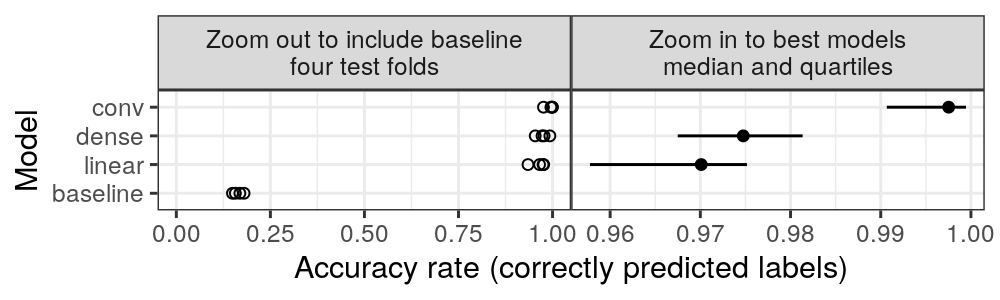
\includegraphics[width=0.8\textwidth]{figure-test-accuracy-both}
  \caption{Prediction accuracy of functions learned for image classification of handwritten digits. The
    baseline function always predicts the most frequent class in the
    train set; other three learned functions are neural
    networks with different numbers of hidden layers (linear=0, conv=2, dense=8).}
  \label{fig:test-accuracy}
\end{figure}

Overall from this comparison it is clear that, among these three
neural networks, the sparse model should be
preferred for most accurate predictions in this particular ``zip''
data set. However, we must be careful to not generalize these
conclusions to other data sets --- even for some other image
classification data sets such as MNIST
(Figure~\ref{fig:drawing-mnist-train-test}), the most accurate
algorithm may be different. For very difficult data sets, it
may even be the case that these three neural networks are no more accurate
than the baseline model which always predicts the most frequent class
in the train set. In general we always need to use computational
cross-validation experiments to determine which machine learning
algorithm is most accurate in any given data set. To learn a
predictive model with maximum prediction accuracy, machine learning
algorithms other than neural networks should be additionally
considered (e.g., regularized linear models, decision trees, random
forests, boosting, support vector machines).

\section{Cross-validation for evaluating predictions of earth system model parameters}

TODO \citep{Feng2020}.

Neural Networking Method

% Both the random-sampling and one-batch methods assume that parameter
% values are spatially homogeneous (constant parameter values across
% the continent). In reality, parameter values in Equation 1 may be
% spatially heterogeneous. We hybridized neural networking with the
% results of site-by-site data assimilation to search for spatially
% heterogeneous parameter values so that modeled SOC can fit best with
% observed SOC. We set the mean values of parameters' posterior
% distributions obtained from the site-by-site data assimilation as
% target parameter values (output in the neural network). By including
% 60 environmental covariates including climate variables and land
% cover types as input, we explored predicting parameter values at
% different sites by a trained neural network. The detailed list of
% environmental covariates, as well as the data sources, are as listed
% in Table S2.

% We designed the neural network as containing four hidden layers with
% backward propagation. The node numbers for each hidden layer were
% 256, 512, 512, and 256. For each hidden layer, the drop ratio was
% set as 0.2. The activation function for hidden layers was RELU. We
% used mean squared error as the loss function and Adadelta as the
% optimizer. Eighty percentage of the results from the site-by-site
% data assimilation were used in training and validating the neural
% network with a validation split ratio of 0.2, and the remaining
% 20% of the site-by-site data assimilation results were used as the testing set. The number of epochs was set as 400, and the batch size was 64. After the neural network training and validation, parameter values for soil sites in the testing set were predicted based on the trained neural network and corresponding auxiliary environmental covariates. The predicted parameter values were then assigned into CLM5 to estimate the SOC content distributions at corresponding sites. Moreover, to represent SOC content distributions for the whole conterminous United States, we used the trained neural network and auxiliary environmental covariate masks of the continent at a resolution of 0.5 degrees to propose parameter values at each grid of the map. The map of SOC content for the conterminous United States was generated by applying the neural network based parameterization into CLM5 matrix model.

\section{Additional reading}

Machine learning is a large field of research with many algorithms,
and there are several useful textbooks that provide overviews from
various perspectives \citep{Bishop2006, Hastie2009, Wasserman2010,
  Murphy2013, Goodfellow2016}.

\paragraph{Reproducibility statement.} Code for figures in this
chapter can be freely downloaded from
\url{https://github.com/tdhock/2020-yiqi-summer-school}

\bibliographystyle{abbrvnat}
\bibliography{refs} 

\end{document}
